%!TEX root = main.tex
\section{Introducción}

El método Monte Carlo es una técnica poderosa y ampliamente utilizada en el transporte de radiación. Su principal ventaja radica en la ausencia de aproximaciones sobre la distribución angular de los flujos de partículas, lo cual asegura una representación fiel incluso en problemas relativamente difíciles, como aquellos con absorbentes fuertes o propagación en vacío.

Un problema de transporte de radiación por Monte Carlo queda esencialmente definido por tres componentes:
\begin{itemize}
    \item Geometría: representación del sistema físico a modelar. Incluye los materiales involucrados y las condiciones de contorno.
    \item Fuente: región donde nacen las partículas, con una dada distribución energética, espacial y angular.
    \item Detector: resultado a obtener de la simulación, usualmente asociado al nivel de flujo o corriente en una región de interés. El cómputo del valor a reportar se realiza en base a las partículas que llegan al detector.
\end{itemize}

La principal dificultad del método Monte Carlo es el relativamente alto costo computacional requerido para obtener resultados confiables. La confiabilidad de un resultado se mide por su varianza estadística, la cual a su vez se relaciona con la cantidad de partículas utilizadas para calcularlo. Para resolver dicha problemática existen diferentes estrategias conocidas como \emph{técnicas de reducción de varianza}, las cuales buscan favorecer la propagación de la radiación hacia la región de interés, respetando la física del problema.

La herramienta KSource permite la implementación de una técnica de reducción de varianza. Por lo tanto, los problemas de interés son situaciones en las cuales no es posible alcanzar estadística suficiente en el detector en una única corrida, pues el costo computacional sería demasiado alto. Desde luego, siempre es posible determinar una superficie más cercana a la fuente en la cual sí es posible alcanzar buena estadística. Dicha situación se esquematiza en la Figura \ref{fig:esq_mc}.

\begin{figure}[htbp!]
    \centering
    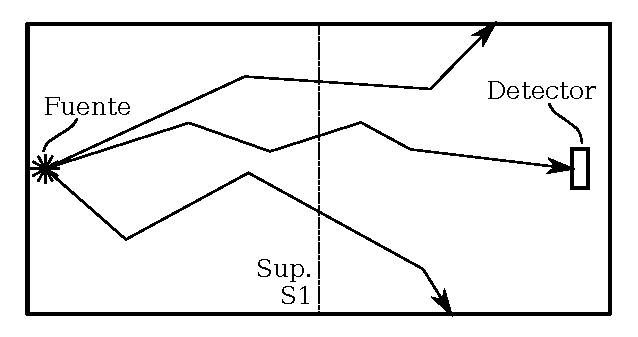
\includegraphics[width=.7\textwidth]{figs/esquema_simul.pdf}
    \caption{Esquema básico de una simulación por Monte Carlo. La superficie S1 permite la implementación de la técnica de reducción de varianza con la herramienta KSource.}
    \label{fig:esq_mc}
\end{figure}

Tomando al problema de la Figura \ref{fig:esq_mc} como ejemplo, el método KSource consiste en registrar las partículas que atraviezan la superficie S1, obteniendo una lista de partículas (energía, posición, dirección) con buena estadística. Luego se utiliza dicha lista para estimar la distribución de corriente en S1, y se utiliza dicha distribución estimada como fuente en una nueva simulación. La cantidad de partículas producidas en esta segunda etapa puede superar el tamaño de la lista original, mejorando la estadística en la región del detector y reduciendo la varianza del resultado. Todo este proceso se muestra en la Figura \ref{fig:esq_rv}. 

\begin{figure}[htbp!]
    \centering
    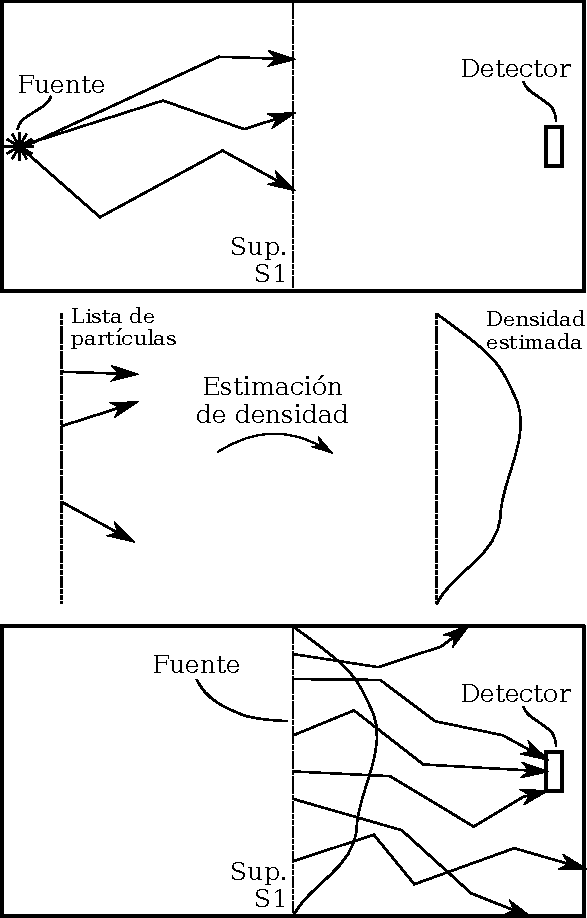
\includegraphics[width=.7\textwidth]{figs/esquema_redvar.pdf}
    \caption{Esquema de la implementación del método KSource. Se utiliza una lista de partículas registrada en una superficie intermedia para estimar su distribución, y utilizar esta última como fuente en una segunda simulación.}
    \label{fig:esq_rv}
\end{figure}


\subsection{\emph{Kernel Density Estimation}}
\label{subsec:kde}

El método empleado para la estimación de densidad es \emph{Kernel Density Estimation} (KDE) [CITA???]. El mismo se basa en la siguiente expresión para la densidad estimada:

\begin{equation}
    \tilde{p}(x) = \frac{1}{N |H|} \sum_{i=1}^N K(H^{-1} (x-x^{(i)}))
    \label{eq:KDE}
\end{equation}
Donde:
\begin{itemize}
    \item $X = \{x^{(i)} \in \mathbb{R}^D\}_{1\leq i \leq N}$ es el conjunto de muestras que representa la lista de partículas.
    \item \tilde{p}(x) es la densidad estimada en función del vector $x=(x_1,...,x_D)$.
    \item $K$ es el \emph{kernel} del método, que en KSource es la distribución normal (\emph{gaussiana}).
    \item $H$ es el ancho de banda (\emph{bandwidth}). En el caso más general considerado en KSource $H=(h_1,...,h_D)$ es un vector, el cual puede ser diferente para cada partícula.
\end{itemize}

Considerando el \emph{kernel} \emph{gaussiano} y el ancho de banda vector la expresión resulta:
\begin{equation}
    Completar...
\end{equation}

El muestreo consiste en obtener nuevas muestras $\tilde{X} = \{\tilde{x}^{(i)} \in \mathbb{R}^D\}_{1\leq i \leq M}$ respetando la densidad estimada en \ref{eq:KDE}. Para el método KDE, la misma se realiza con el siguiente algoritmo:
\begin{itemize}
    \item Se toma un $x^{(i)} \in X$.
    \item Se obtiene la nueva muestra como $x = x^{(i)} + \Delta$, siendo $\Delta$ una perturbación aleatoria con la distribución del \emph{kernel} (\emph{gaussiana}) y los anchos de banda correspondientes a $x^{(i)}$.
\end{itemize}
Al repetir el muestreo, los $x^{(i)}$ se van tomando en orden tal como están en la lista de partículas. Cuando se llega al final, se vuelve al principio.

El ancho de banda es el parámetro más importante del método KDE. Para que la estimación de densidad tenga el mínimo error posible, los anchos de banda deben ser optimizados. Para ello KSource incluye tres métodos:
\begin{itemize}
    \item Regla de Silverman [CITA??]
    \item K Vecinos Más Cercanos (KNN) [CITA??]
    \item Validación cruzada
\end{itemize}